\section{Introduction}

This is the latex template for the ReScience journal
\citep{Rougier:2017}\sidecite{Rougier:2017}, {\em a peer-reviewed
journal that targets computational research and encourages the explicit
replication of already published research, promoting new and open-source
implementations in order to ensure that the original research is
reproducible.}\\


\subsection*{Font stack}
\marginnote{%
  
\begin{tikzpicture}
    \node[draw, fill=black!5, dashed, thick,
          text width=\marginparwidth, minimum height=3cm] at (0,0) {~~\sf Figure 1};
  \end{tikzpicture}
  \captionof{figure}{Side figure using and caption}}
Test
\begin{description}
\item[{\bfseries Serif font}] The
  \href{http://www.tug.dk/FontCatalogue/urwpalladio}{Pazo Math fonts} are a
  family of PostScript fonts suitable for typesetting mathematics in
  combination with the Palatino family of text fonts.
\item[{\sf \bfseries Sans Serif}] The
  \href{http://www.tug.dk/FontCatalogue/firasans/}{Fira Sans fonts} is a
  humanist sans-serif typeface designed by Erik Spiekermann, Ralph du Carrois,
  Anja Meiners and Botio Nikoltchev of Carrois Type Design for the Firefox OS.
\item[{\tt \bfseries Monotype}]
  \href{http://www.tug.dk/FontCatalogue/inconsolata/}{Inconsolata} is
  amonospaced font designed by Raph Levien and has regular and bold weights,
  with additional glyphs and options to control slashed zero, upright quotes
  and a shapelier lower-case L.
\end{description}

An article is composed of four different files:
\begin{lstlisting}
article-metadata.tex
article-header.tex
article-content.tex
article-bibliography.bib
\end{lstlisting}


The {\tt article-metadata.tex} file is generated by the {\tt generate-latex.py}.\\

%% \begin{minipage}{\headwidth}
%%   \begin{framed}
%%     \em \lipsum[1]
%%   \end{framed}
%% \end{minipage}


%% \marginnote{
%% \begin{figure}[htbp]
%%   \caption{Full width figure ({\tt width=\textbackslash headwidth}) uses a
%%     regular caption}
%%   \label{fig:1}
%% \end{figure}
%% }

\begin{figure}[htbp]
  \marginnote{
    \caption{Side caption can be easily inserted using the {\tt \textbackslash
        marginnote} command. Note that you may have to slightly adjust the
      vertical offset to align caption and the top of figure which is the
      recommended layout.}}[-2.5em]
  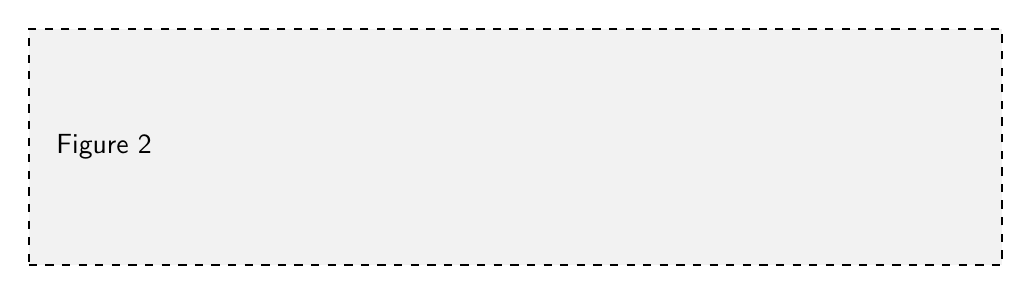
\begin{tikzpicture}
    \node[draw, fill=black!5, dashed, thick,
          text width=\textwidth, minimum height=3cm] at (0,0) {~~\sf Figure 2};
  \end{tikzpicture}
  \label{fig:2}
\end{figure}

%% \begin{figure}[htbp]
%%   \begin{tikzpicture}
%%     \node[draw, fill=black!5, dashed, thick,
%%           text width=.99\headwidth, minimum height=3cm] at (0,0) {~~\sf Figure 3};
%%   \end{tikzpicture}
%%   \marginnote{
%%     \caption{Full width figure using a side caption Lorem ipsum dolor sit amet, consectetuer adipiscing elit.}}[-2.0em]
%%   \label{fig:3}
%% \end{figure}

\section{Commands}

The template defines various commands to help with the writing.
\begin{lstlisting}
\citep{Rougier:2017}\sidecite{Rougier:2017}
\end{lstlisting}

\lipsum[3]

